The Reporting module represents the core of the value that the users will
get out of the system. Reports are the means with which the users will
be able to see the results of the benchmarking of their programs.

\subsection{Scope}
The scope for the reporting module is shown in Figure \ref{Reporting Scope}
\begin{figure}[H]
  \begin{center}
  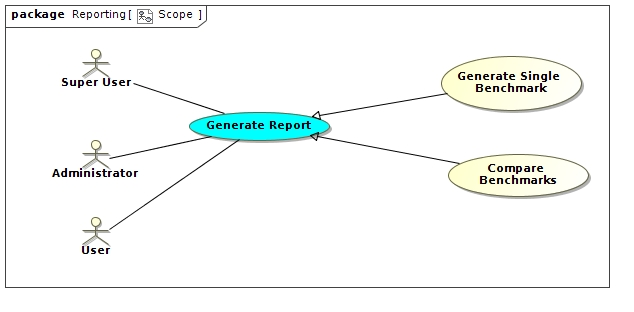
\includegraphics[scale=0.7]{../Diagrams and Charts/Reporting/Scope.jpg}
  \caption{Reporting Scope}
  \end{center}
  \label{Reporting Scope}
\end{figure}

The scope of the reporting module include:
\begin{itemize}
	\item The ability to genretate a report on a single benchmark
	\item The ability to generate a report that will compare more than
	two or more benchmarks
\end{itemize}

\subsection{Domain Model}
